\documentclass{standalone}
\usepackage{tikz}
\usetikzlibrary{patterns, positioning}
\usepackage[sfdefault]{ClearSans} %% option 'sfdefault' activates Clear Sans as the default text font
\usepackage[T1]{fontenc}

\begin{document}
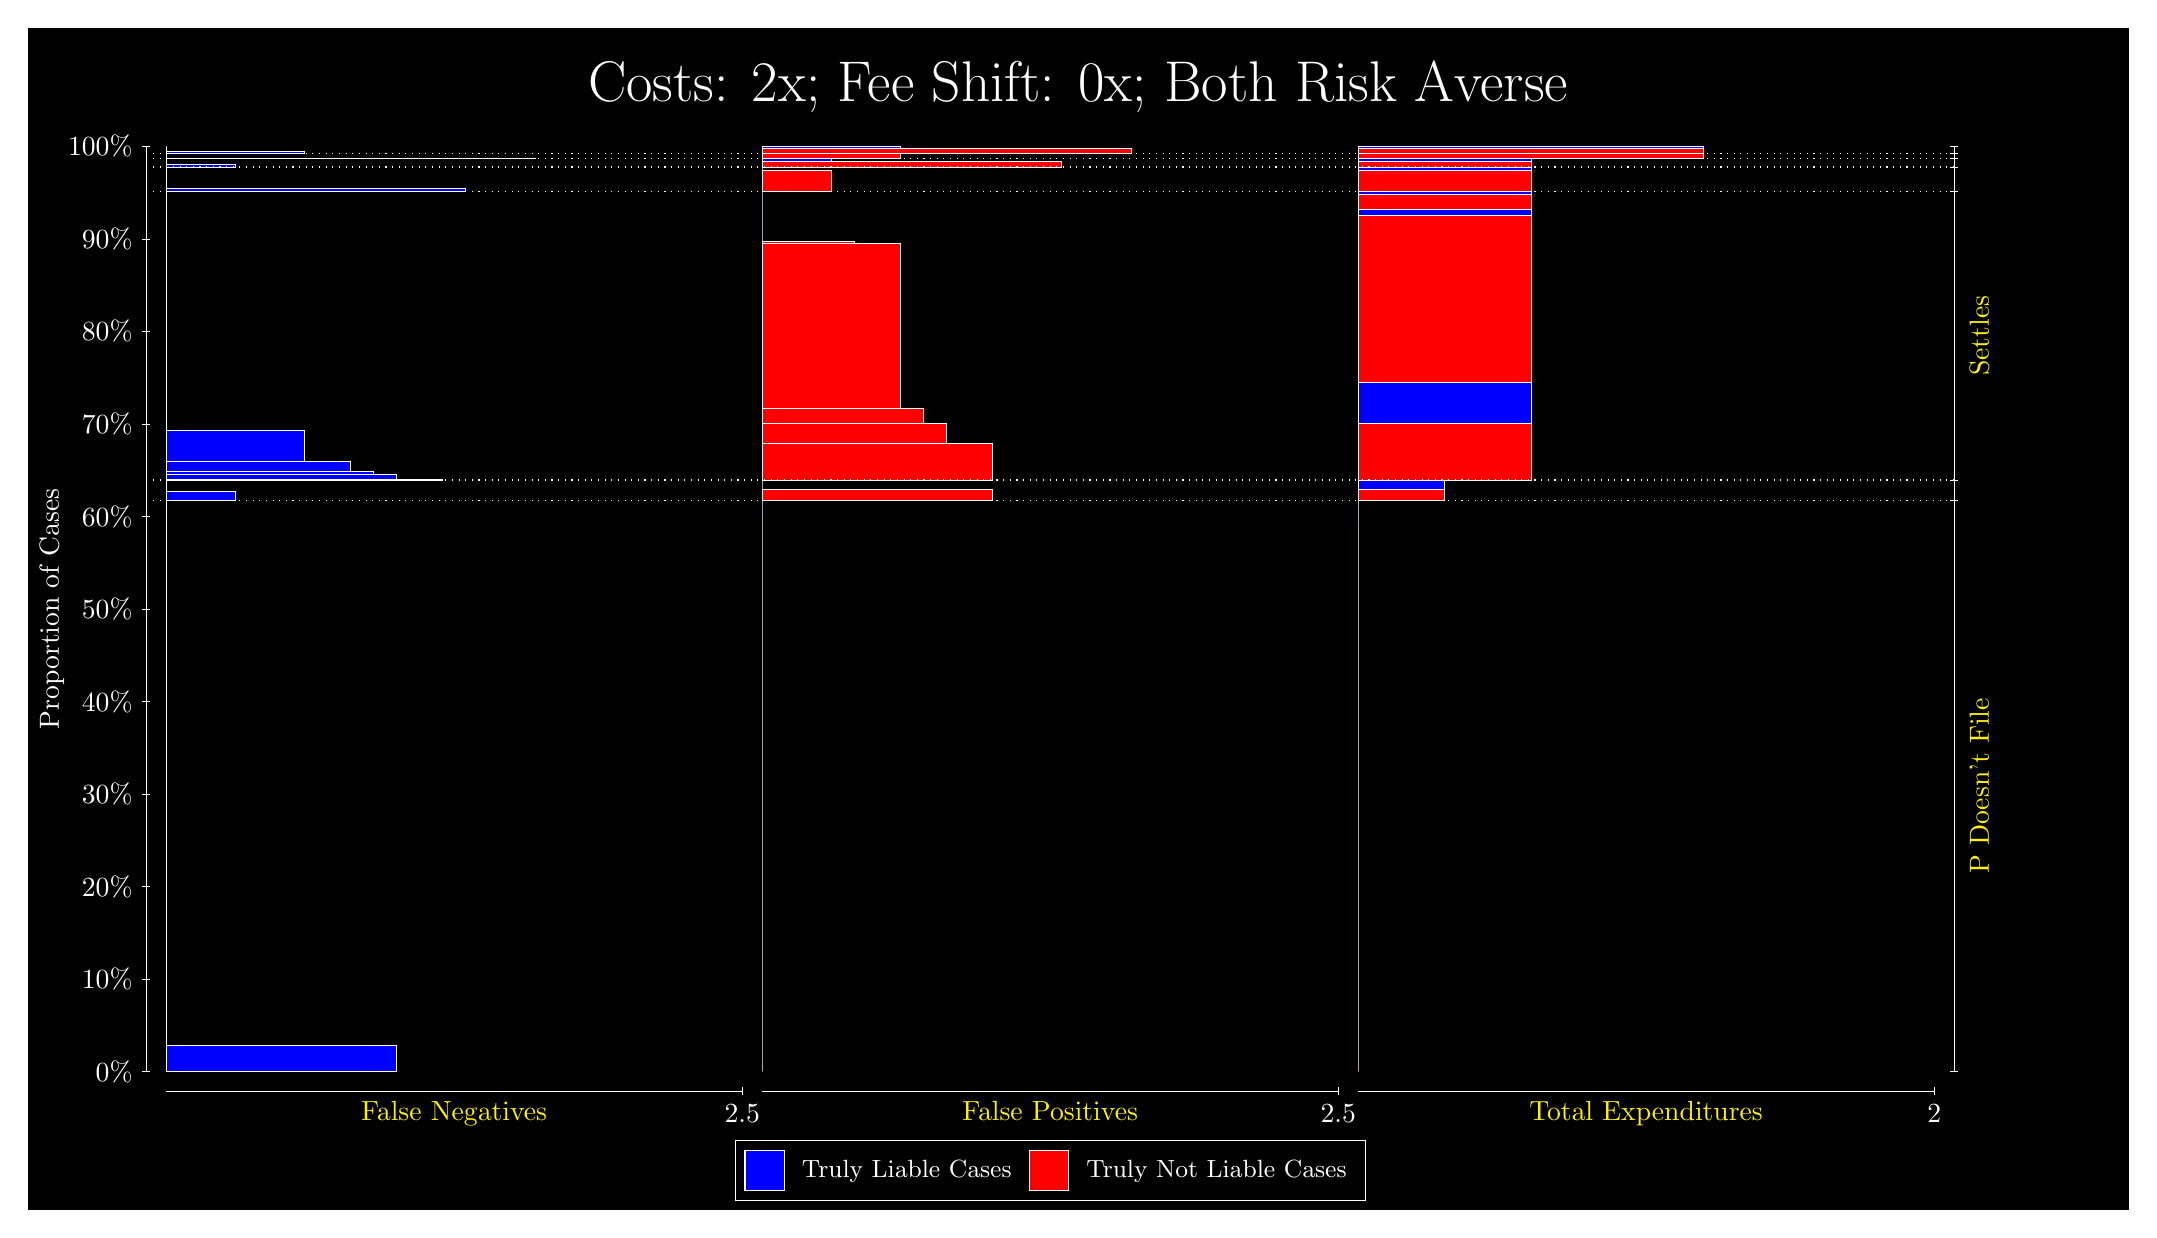
\begin{tikzpicture}
\draw[fill=black] (0,0) rectangle (26.667,15);
\draw[text=white] (0,13.5) rectangle (26.667,15) node[midway] {\huge Costs: 2x; Fee Shift: 0x; Both Risk Averse};
\draw[white, very thin] (1.5,1.75) -- (1.5,13.5);
\node[rotate=90, text=white, anchor=center] at (0.3, 7.625) {Proportion of Cases};
\draw[white, very thin] (1.45,1.75) -- (1.55,1.75);
\node[text=white, anchor=east] at (1.45, 1.75) {0\%};
\draw[white, very thin] (1.45,2.925) -- (1.55,2.925);
\node[text=white, anchor=east] at (1.45, 2.925) {10\%};
\draw[white, very thin] (1.45,4.1) -- (1.55,4.1);
\node[text=white, anchor=east] at (1.45, 4.1) {20\%};
\draw[white, very thin] (1.45,5.275) -- (1.55,5.275);
\node[text=white, anchor=east] at (1.45, 5.275) {30\%};
\draw[white, very thin] (1.45,6.45) -- (1.55,6.45);
\node[text=white, anchor=east] at (1.45, 6.45) {40\%};
\draw[white, very thin] (1.45,7.625) -- (1.55,7.625);
\node[text=white, anchor=east] at (1.45, 7.625) {50\%};
\draw[white, very thin] (1.45,8.8) -- (1.55,8.8);
\node[text=white, anchor=east] at (1.45, 8.8) {60\%};
\draw[white, very thin] (1.45,9.975) -- (1.55,9.975);
\node[text=white, anchor=east] at (1.45, 9.975) {70\%};
\draw[white, very thin] (1.45,11.15) -- (1.55,11.15);
\node[text=white, anchor=east] at (1.45, 11.15) {80\%};
\draw[white, very thin] (1.45,12.325) -- (1.55,12.325);
\node[text=white, anchor=east] at (1.45, 12.325) {90\%};
\draw[white, very thin] (1.45,13.5) -- (1.55,13.5);
\node[text=white, anchor=east] at (1.45, 13.5) {100\%};

\draw[white, very thin] (24.457,1.75) -- (24.457,13.5);
\draw[white, very thin] (24.407,1.75) -- (24.507,1.75);
\node[anchor=west] at (24.407, 1.75) {};
\draw[white, very thin] (24.407,9.0013) -- (24.507,9.0013);
\node[anchor=west] at (24.407, 9.0013) {};
\draw[white, very thin] (24.407,9.2624) -- (24.507,9.2624);
\node[anchor=west] at (24.407, 9.2624) {};
\draw[white, very thin] (24.407,12.926) -- (24.507,12.926);
\node[anchor=west] at (24.407, 12.926) {};
\draw[white, very thin] (24.407,13.237) -- (24.507,13.237);
\node[anchor=west] at (24.407, 13.237) {};
\draw[white, very thin] (24.407,13.344) -- (24.507,13.344);
\node[anchor=west] at (24.407, 13.344) {};
\draw[white, very thin] (24.407,13.414) -- (24.507,13.414);
\node[anchor=west] at (24.407, 13.414) {};
\draw[white, very thin] (24.407,13.5) -- (24.507,13.5);
\node[anchor=west] at (24.407, 13.5) {};

\draw[white, very thin, fill=blue] (1.75,1.75) rectangle (4.6775,2.08);
\draw[white, very thin, fill=red] (1.75,2.08) rectangle (1.75,9.0013);
\draw[white, very thin, fill=blue] (1.75,9.0013) rectangle (2.6283,9.115);
\draw[white, very thin, fill=red] (1.75,9.115) rectangle (1.75,9.2624);
\draw[white, very thin, fill=blue] (1.75,9.2624) rectangle (5.2631,9.2661);
\draw[white, very thin, fill=blue] (1.75,9.2661) rectangle (4.6775,9.3363);
\draw[white, very thin, fill=blue] (1.75,9.3363) rectangle (4.3848,9.3702);
\draw[white, very thin, fill=blue] (1.75,9.3702) rectangle (4.092,9.4953);
\draw[white, very thin, fill=blue] (1.75,9.4953) rectangle (3.5065,9.892);
\draw[white, very thin, fill=red] (1.75,9.892) rectangle (1.75,12.926);
\draw[white, very thin, fill=blue] (1.75,12.926) rectangle (5.5558,12.963);
\draw[white, very thin, fill=red] (1.75,12.963) rectangle (1.75,13.237);
\draw[white, very thin, fill=blue] (1.75,13.237) rectangle (2.6283,13.269);
\draw[white, very thin, fill=red] (1.75,13.269) rectangle (1.75,13.344);
\draw[white, very thin, fill=blue] (1.75,13.344) rectangle (6.4341,13.351);
\draw[white, very thin, fill=red] (1.75,13.351) rectangle (1.75,13.414);
\draw[white, very thin, fill=blue] (1.75,13.414) rectangle (3.5065,13.44);
\draw[white, very thin, fill=red] (1.75,13.44) rectangle (1.75,13.5);
\draw[white, very thin, fill=red] (9.3189,1.75) rectangle (9.3189,8.6713);
\draw[white, very thin, fill=blue] (9.3189,8.6713) rectangle (9.3189,9.0013);
\draw[white, very thin, fill=red] (9.3189,9.0013) rectangle (12.246,9.1487);
\draw[white, very thin, fill=blue] (9.3189,9.1487) rectangle (9.3189,9.2624);
\draw[white, very thin, fill=red] (9.3189,9.2624) rectangle (12.246,9.7327);
\draw[white, very thin, fill=red] (9.3189,9.7327) rectangle (11.661,9.98);
\draw[white, very thin, fill=red] (9.3189,9.98) rectangle (11.368,10.171);
\draw[white, very thin, fill=red] (9.3189,10.171) rectangle (11.075,12.264);
\draw[white, very thin, fill=red] (9.3189,12.264) rectangle (10.49,12.296);
\draw[white, very thin, fill=blue] (9.3189,12.296) rectangle (9.3189,12.926);
\draw[white, very thin, fill=red] (9.3189,12.926) rectangle (10.197,13.2);
\draw[white, very thin, fill=blue] (9.3189,13.2) rectangle (9.3189,13.237);
\draw[white, very thin, fill=red] (9.3189,13.237) rectangle (13.125,13.312);
\draw[white, very thin, fill=blue] (9.3189,13.312) rectangle (10.197,13.344);
\draw[white, very thin, fill=red] (9.3189,13.344) rectangle (11.075,13.407);
\draw[white, very thin, fill=blue] (9.3189,13.407) rectangle (9.3189,13.414);
\draw[white, very thin, fill=red] (9.3189,13.414) rectangle (14.003,13.475);
\draw[white, very thin, fill=blue] (9.3189,13.475) rectangle (11.075,13.5);
\draw[white, very thin, fill=red] (16.888,1.75) rectangle (16.888,8.6713);
\draw[white, very thin, fill=blue] (16.888,8.6713) rectangle (16.888,9.0013);
\draw[white, very thin, fill=red] (16.888,9.0013) rectangle (17.986,9.1487);
\draw[white, very thin, fill=blue] (16.888,9.1487) rectangle (17.986,9.2624);
\draw[white, very thin, fill=red] (16.888,9.2624) rectangle (19.083,9.98);
\draw[white, very thin, fill=blue] (16.888,9.98) rectangle (19.083,10.502);
\draw[white, very thin, fill=red] (16.888,10.502) rectangle (19.083,12.627);
\draw[white, very thin, fill=blue] (16.888,12.627) rectangle (19.083,12.701);
\draw[white, very thin, fill=red] (16.888,12.701) rectangle (19.083,12.892);
\draw[white, very thin, fill=blue] (16.888,12.892) rectangle (19.083,12.926);
\draw[white, very thin, fill=red] (16.888,12.926) rectangle (19.083,13.2);
\draw[white, very thin, fill=blue] (16.888,13.2) rectangle (19.083,13.237);
\draw[white, very thin, fill=red] (16.888,13.237) rectangle (19.083,13.312);
\draw[white, very thin, fill=blue] (16.888,13.312) rectangle (19.083,13.344);
\draw[white, very thin, fill=red] (16.888,13.344) rectangle (21.279,13.407);
\draw[white, very thin, fill=blue] (16.888,13.407) rectangle (21.279,13.414);
\draw[white, very thin, fill=red] (16.888,13.414) rectangle (21.279,13.475);
\draw[white, very thin, fill=blue] (16.888,13.475) rectangle (21.279,13.5);
\draw[white, dotted] (1.5,9.0013) -- (24.457,9.0013);
\draw[white, dotted] (1.5,9.2624) -- (24.457,9.2624);
\draw[white, dotted] (1.5,12.926) -- (24.457,12.926);
\draw[white, dotted] (1.5,13.237) -- (24.457,13.237);
\draw[white, dotted] (1.5,13.344) -- (24.457,13.344);
\draw[white, dotted] (1.5,13.414) -- (24.457,13.414);
\draw[white, very thin] (1.75,1.5) -- (9.0689,1.5);
\node[text=yellow, anchor=north] at (5.4094, 1.5) {False Negatives};
\draw[white, very thin] (9.0689,1.45) -- (9.0689,1.55);
\node[text=white, anchor=north] at (9.0689, 1.45) {2.5};

\draw[white, very thin] (9.3189,1.5) -- (16.638,1.5);
\node[text=yellow, anchor=north] at (12.978, 1.5) {False Positives};
\draw[white, very thin] (16.638,1.45) -- (16.638,1.55);
\node[text=white, anchor=north] at (16.638, 1.45) {2.5};

\draw[white, very thin] (16.888,1.5) -- (24.207,1.5);
\node[text=yellow, anchor=north] at (20.547, 1.5) {Total Expenditures};
\draw[white, very thin] (24.207,1.45) -- (24.207,1.55);
\node[text=white, anchor=north] at (24.207, 1.45) {2};

\node[text=yellow, centered, rotate=90] at (24.777, 5.3757) {P Doesn't File};

\node[text=yellow, centered, rotate=90] at (24.777, 11.094) {Settles};





\draw (12.978300999999998,1.5) node[draw=none] (baseCoordinate) {};
\begin{scope}[align=center]
        \matrix[scale=0.5, draw=white, below=0.5cm of baseCoordinate, nodes={draw}, column sep=0.1cm]{
            \node[rectangle, draw, minimum width=0.5cm, minimum height=0.5cm, fill=blue] {}; &
            \node[draw=none, font=\small, text=white] (B) {Truly Liable Cases}; &
            \node[rectangle, draw, minimum width=0.5cm, minimum height=0.5cm, fill=red] {}; &
            \node[draw=none, font=\small, text=white] (B) {Truly Not Liable Cases}; \\
            };
\end{scope}

\end{tikzpicture}
\end{document}